\section{pset1}

\subsection{a}
    It is possible that the third option c could be true. This is because we see an exponential acceleration in the Y direction, which correlates with \(W^2\)

\subsection{b}
    \[a = F \quad t = \frac{L}{V_0} \rightarrow y_f = \frac{1}{2}\frac{F L^2}{V_0}\]

\subsection{c}
    \[\frac{w}{2} =\frac{1}{2} \frac{F_{max} L^2}{mv_0^2} \qquad F_{max} = \frac{mv_0^2w}{L^2}\]
\subsection{d}
    \[tan(\theta) = \frac{v_y}{v_o} = \frac{w}{l}\]
    \[v_y = 
    \frac{F}{m} \times \frac{L}{v_0}\]
\section{}
\subsection{}
    It has a net force of 0. This is because the x and y components cancel each other out. 
\subsection{}
    The y component would cancel, as it is symmetric around the particle. X would not 
    form a triangle to find r to use \(u_g = \frac{-Gm_1m_2}{r^2}\)

    \[F_g = -\frac{GMm}{{(\frac{\sqrt{5a}}{2})}^2}\]

    % \[F_g = -\frac{GMm}{\sqrt{5a}}{2}\]
    \[F_{g,x} = -\frac{16Mm}{g\sqrt{g}a^2}\]

    % \[F_{g,x} = -\frac{GMm}{a^2}\]

\subsection{}

\subsection{}
    The physical argument is that the object is quite far away, and thus we can use a small angle aprox. 

    \[\sqrt{(x-a/2)^2+(a/2)^2} \rightarrow \approx x\]

    \[{\frac{GMm}{x^2}}\]
\section{RL stuff lol}
    it is the fourth one

    \subsection{}
    \[u_c = -\frac{4\sqrt{2}GMm}{a}\]
    \subsection{}
    \[\Delta u = \frac{4\sqrt{2}GMm}{a} = \frac{1}{2}mv^2\]
    \[v = \sqrt{\frac{8\sqrt{2}GM}{a}}\]
    \subsection{}
    \[u_1, u_2 = -\frac{2GMm}{a}\]
    \[u_3, u_4 = \frac{-2GMm}{\sqrt{5}a}\]
    \[u= u_1 +u_2 \dots = -\frac{4GMm}{a} (1+\frac{1}{\sqrt{5} = Ur})\]

    \subsection{} 
    no, the middle has \textit{higher} potential energy

    \subsection{}

\section{}
    \subsection{}
    \[p^2 = \frac{4a^3\pi^2}{GM}\]
    \subsection{}
    \[\omega = 2\pi/p \rightarrow \omega^2 = \frac{\cancel{4\pi^2} GM}{\cancel{4a}^3\cancel{\pi^2}} = \frac{GM}{r^3}\]
    \subsection{}
    \[Dw^aR6{a+b}\]
    \[a = \frac{D}{m} w^a R^{a+b} = \omega^2R\]
    \[\omega^{2-a} = \frac{D}{m}R^{a+b-1}\]
    \subsection{}
    
    
\pagebreak
\section{w2}
\hrule
\vspace{.5cm}

\subsection{q1}

\begin{example}
\begin{center}
        The configuration below shows some points
    around a positive charge Q. If a positive test charge q
    is placed at point A, at a distance rA from Q, calculate
    the magnitude of the force between the charges in
    terms the given variables. \\

    \vspace{.5cm}
    % \begin{tikzpicture}[scale=1.2]
    
    % % Central charge
    % \draw[fill=black!50] (0,0) circle (0.5);
    % \node at (0,0) {\Large $Q$};
    % \node[pt] (A) at (0,-2) {};
    % \node[pt] (B) at (1.6,0.2) {};
    % \node[pt] (C) at (3.3,0.25) {};
    % \node[pt] (D) at (-3.2,0.1) {};
    
    % % Points
    % \fill (-3,0) circle (2pt) node[left] {$D$};
    % \fill (1.6,0.2) circle (2pt) node[right] {$B$};
    % \fill (3.0,0.3) circle (2pt) node[right] {$C$};
    % \fill (0,-2.0) circle (2pt) node[below] {$A$};

    % \draw[->, white, line width=1pt] (A) -- ++(0,1.5);

    
    % \end{tikzpicture}


    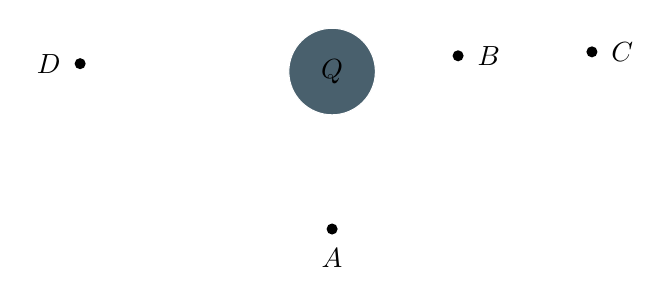
\begin{tikzpicture}

    \node[label={below:$A$}] (A) at (0,-2) {};
    \node[label={right:$B$}] (B) at (1.6,0.2) {};
    \node[label={right:$C$}] (C) at (3.3,0.25) {};
    \node[label={left:$D$}]  (D) at (-3.2,0.1) {};

    \fill (A) circle (2pt);
    \fill (B) circle (2pt);
    \fill (C) circle (2pt);
    \fill (D) circle (2pt);

    \node[draw=white, fill=cyan!35!black, circle, minimum size=1.1cm] (Q) at (0,0) {$Q$};

    % arrows plotted using nodes
    \draw[->, white, thick] (A) -- ++(0,.5);
    \draw[->, white, thick] (Q) -- ++(0,-1);
    
    \draw[->, white, thick] (B) -- ++(-.75,0);
    \draw[->, white, thick] (C) -- ++(-.4,0);
    \draw[->, white, thick] (D) -- ++(.3,0);
    
    \end{tikzpicture}

    \hrulefill \vspace{.5cm }\\ \textbf{P1) Find magnitude}
    
    Because we're finding a charge diff, we use \ref{eq:CoulombsLaw}
    \[\vec{F_{12}} = k \frac{Qq}{r_A^2}\]

    \hrulefill \vspace{.5cm }\\ \textbf{P2) Force strength}

    Based on distance to the \textit{field} of Q  
    \[F_B > F_A > F_C > F_D\]

    \hrulefill \vspace{.5cm }\\ \textbf{P4) Electric Field Mag}

    Because a test charge placed in a field exerts doesn't have any force of its own, we use a modified version of \ref{eq:ElectricField}

    \[E = k \frac{Q}{r_a^2}\]

    Based on above\dots 
    \[2Q \propto 2E, \quad 2q \cancel{\propto} 2E\] 
    
\end{center}
\end{example}

\pagebreak

\hrule
\begin{example}
\begin{center}
\textbf{Electric Field Due to Point Charges}
Four point charges 2q, q, q, and q are placed at the corners of a rectangle of dimensions a and 3a as shown in the figure. A fifth charge Q is placed at the center of the rectangle. Our task is to compute the electric field at the center of the rectangle, and then determine the force on Q.

\begin{tikzpicture}
    \node[label={above left:  $q$}] (A) at (-6, 2) {};
    \node[label={above right :$2q$}] (B) at (6 ,2 ) {};
    \node[label={below left:  $q$}] (C) at (-6,-2) {};
    \node[label={below right: $q$}] (D) at (6 ,-2) {};

    \fill (A) circle (2pt);
    \fill (B) circle (2pt);
    \fill (C) circle (2pt);
    \fill (D) circle (2pt);

  % \\draw[->, white, thick] (A) -- ++(0,${11:1});",
    \draw[-, white, thick] (A) -- ++(B) node[midway, above] {$3a$};
    \draw[-, white, thick] (C) -- ++(A) node[midway, left] {$a$};
    \draw[-, white, thick] (C) -- ++(D);
    \draw[-, white, thick] (D) -- ++(B);
    \draw[-, white, dashed](C) -- ++(B);
    
    \node[draw=white, fill=cyan!35!black, circle, minimum size=.4cm] (Q) at (0,0) {$Q$}; 


\end{tikzpicture}

    \hrulefill \vspace{.5cm }\\ \textbf{P1) Find the mag of field charges}
    \[r = \sqrt{\left(\frac{3a}{2}\right)^2 + \frac{1}{(2a)^2}}\]
    \[r = \sqrt{\frac{9a^2}{4} + \frac{1}{4a^2}}\] 
    \[r = \sqrt{\left(\frac{10a^2}{4}\right)}\]
    \[r = \frac{\sqrt{5}}{\sqrt{2}}a \]
    \[q = E_1 = \frac{2ka}{5a^2}, \quad 2q = E_2 = \frac{4ka}{5a^2}\]
    
    \hrulefill \vspace{.5cm } \\ \textbf{P3) Find X and Y components}


\end{center}
\end{example}


\pagebreak
\section{D4}
\hrule
\vspace{.5cm}


\begin{example}
    \begin{center}
        \textbf{Electric Potential in a System with Cylindrical Symmetry}
    \vspace{.2cm}
    
    \hrule
    \vspace{.5cm}

    \begin{tikzpicture}
    % Outer shell shading
    \draw[gray!80, pattern=north east lines, pattern color = white!50!black] (0,0) circle (2.5cm);
    \fill[black!85] (0,0) circle (1.8cm);
    \draw (0,0) circle (1.8cm);
    \draw (0,0) circle (2.5cm);

    
    % Inner cylinder
    \fill[blue!80] (0,0) circle (1cm);
    \draw (0,0) circle (1cm);
    
    % Labels and vectors
    \draw[->] (0,0) -- (30:1cm) node[midway, below] {$a$};
    \draw[->] (0,0) -- (110:1.8cm) node[midway, above left] {$b_1$};
    \draw[->] (0,0) -- (150:2.5cm) node[midway, below left] {$b_2$};
    
    \node at (0,-0.3) {$\rho$};
    \node[align=right] at (4, 0) {conducting shell, \\ uncharged};
    \draw[->] (3.2, -0.2) -- (2.1, -0.5);
    
    \node[align=left] at (-3.3, -1) {$V=0$};
    \draw[->] (-2.7, -1) -- (-2.4, -.95);

    \node at (4, 2) {
        \boxed{
            \begin{tabular}{r}
                $a = 3 \text{cm}$ \\
                $b_1 = 6 \text{cm}$ \\
                $b_2 = 8 \text{cm}$ \\
                $\rho = +7.5 \text{ C/m}^3$
            \end{tabular}
        }
    };

    \end{tikzpicture}

    \textbf{Find the potential at r = 10cm}

    Find the energy enclosed using Gauss's Law ({\ref{eq:GausssLaw})
    }
    \[\int \vec{E} dS = \frac{Q_{enc}}{\epsilon_0}\]
    \[
    \lambda = \rho * \pi *a^2
    \]
    \[
    Q_{enc} = \rho \pi a^2 L 
    \]
    \[
    E (2\cancel{\pi} r) = \rho \cancel{\pi} a^2
    \]
    \[
    E = \frac{\rho a^2 }{2\epsilon_0 r}
    \]
    \[
    V(r) = \int_r^{b_2} \frac{\rho a^2 }{2\epsilon_0 r}
    \]
    \[
    V(r) = \frac{\rho a^2 }{2\epsilon_0}\ln\left(\frac{b_2}{r}\right)
    \]
    

    \end{center}

    


\end{example}